\documentclass[tikz,border=10pt]{standalone}

\usepackage{amsmath,amssymb}
\usepackage{tikz}
\usetikzlibrary{arrows.meta,positioning,calc}

\newcommand{\F}{\mathbb{F}}
\newcommand{\C}{\mathbb{C}}
\newcommand{\Z}{\mathbb{Z}}
\newcommand{\Spec}{\operatorname{Spec}}

\begin{document}
	
	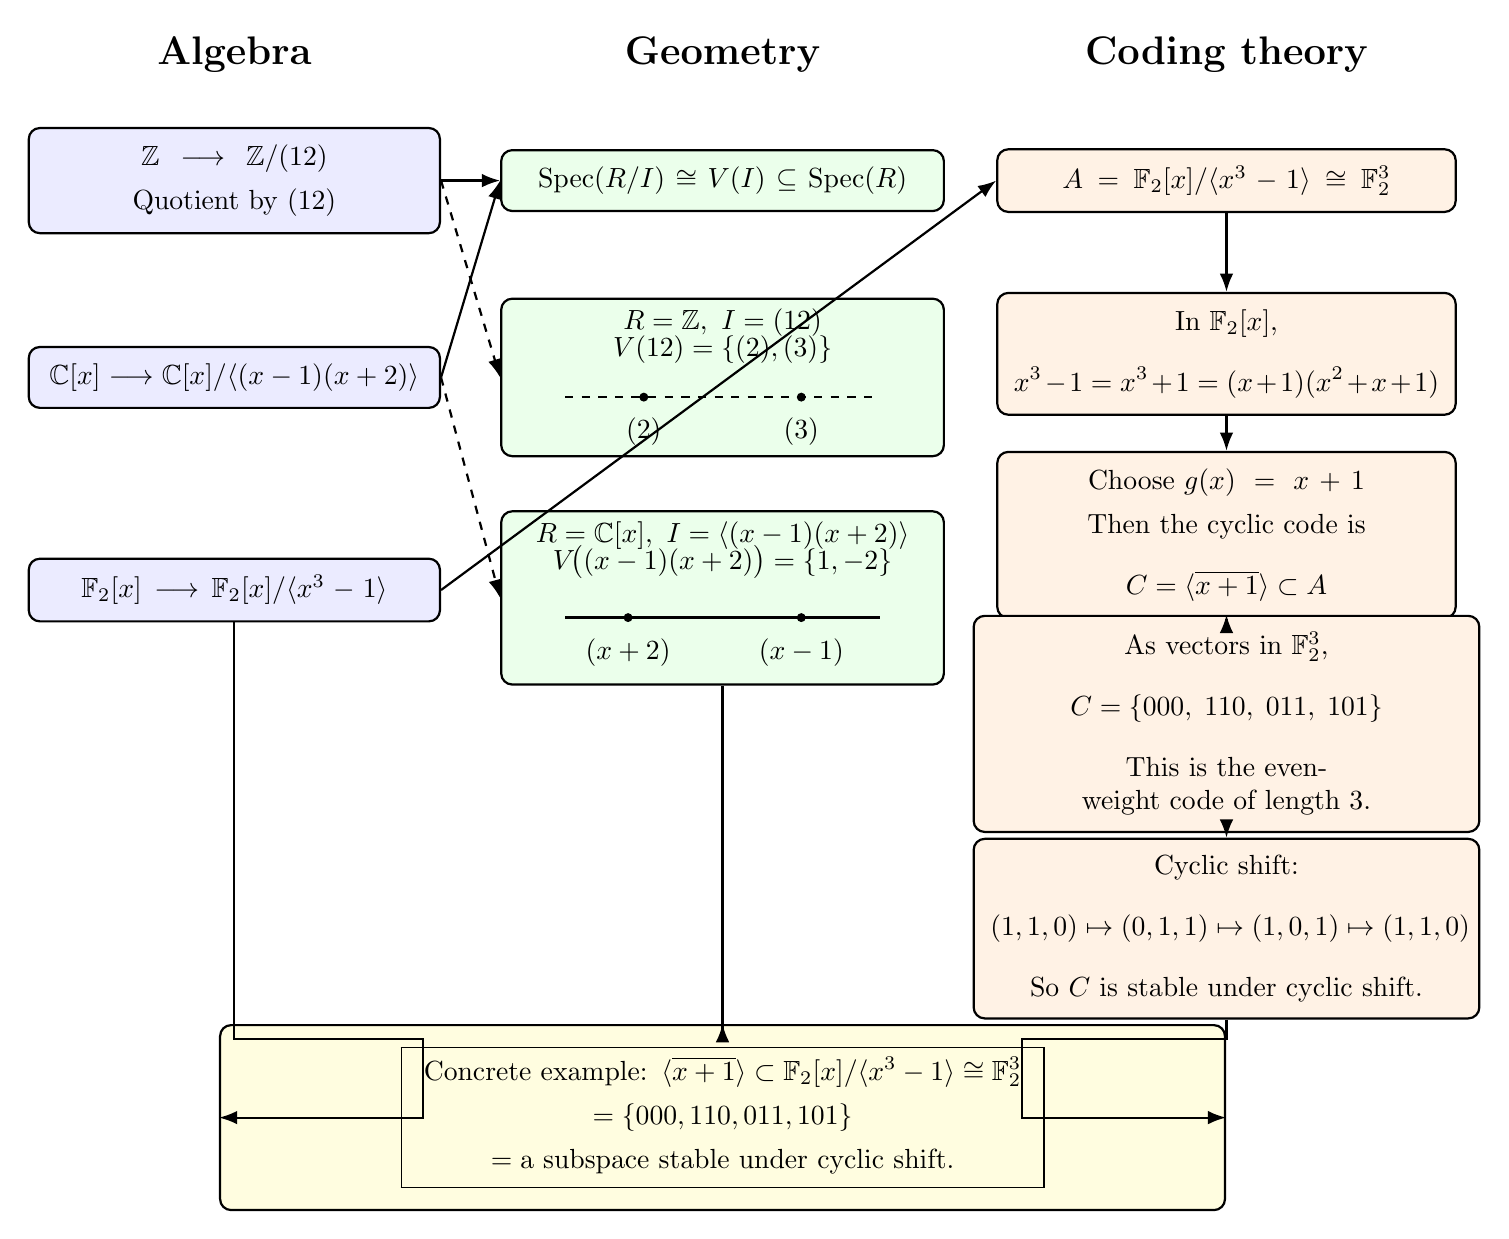
\begin{tikzpicture}[
		>=Latex,
		box/.style={draw, rounded corners, thick, align=center, inner sep=6pt},
		alg/.style={box, fill=blue!8, text width=4.8cm},
		geo/.style={box, fill=green!8, text width=5.2cm},
		code/.style={box, fill=orange!10, text width=5.4cm},
		sum/.style={box, fill=yellow!12, text width=12.2cm, inner sep=8pt}
		]
		
		% Titles
		\node[font=\bfseries\Large] at (-6.2,5.3) {Algebra};
		\node[font=\bfseries\Large] at (0,5.3) {Geometry};
		\node[font=\bfseries\Large] at (6.4,5.3) {Coding theory};
		
		% -------------------------
		% Algebra column
		% -------------------------
		\node[alg] (A1) at (-6.2,3.7) {%
			$\Z \longrightarrow \Z/(12)$\\[4pt]
			Quotient by $(12)$
		};
		
		\node[alg] (A2) at (-6.2,1.2) {%
			$\C[x]\longrightarrow \C[x]/\langle (x-1)(x+2)\rangle$
		};
		
		\node[alg] (A3) at (-6.2,-1.5) {%
			$\F_2[x]\longrightarrow \F_2[x]/\langle x^3-1\rangle$
		};
		
		% -------------------------
		% Geometry column
		% -------------------------
		\node[geo] (G0) at (0,3.7) {%
			$\Spec(R/I)\cong V(I)\subseteq \Spec(R)$
		};
		
		\node[geo, minimum height=2.0cm] (G1) at (0,1.2) {};
		\node at ($(G1.north)+(0,-0.32)$) {$R=\Z,\ I=(12)$};
		\draw[dashed, thick] ($(G1.center)+(-2.0,-0.25)$) -- ($(G1.center)+(2.0,-0.25)$);
		\filldraw[black] ($(G1.center)+(-1.0,-0.25)$) circle (1.4pt);
		\filldraw[black] ($(G1.center)+( 1.0,-0.25)$) circle (1.4pt);
		\node[below=4pt] at ($(G1.center)+(-1.0,-0.25)$) {$(2)$};
		\node[below=4pt] at ($(G1.center)+(1.0,-0.25)$) {$(3)$};
		\node at ($(G1.center)+(0,0.35)$) {$V(12)=\{(2),(3)\}$};
		
		\node[geo, minimum height=2.2cm] (G2) at (0,-1.6) {};
		\node at ($(G2.north)+(0,-0.32)$) {$R=\C[x],\ I=\langle (x-1)(x+2)\rangle$};
		\draw[thick] ($(G2.center)+(-2.0,-0.25)$) -- ($(G2.center)+(2.0,-0.25)$);
		\filldraw[black] ($(G2.center)+(-1.2,-0.25)$) circle (1.4pt);
		\filldraw[black] ($(G2.center)+( 1.0,-0.25)$) circle (1.4pt);
		\node[below=4pt] at ($(G2.center)+(-1.2,-0.25)$) {$(x+2)$};
		\node[below=4pt] at ($(G2.center)+(1.0,-0.25)$) {$(x-1)$};
		\node at ($(G2.center)+(0,0.45)$) {$V\!\bigl((x-1)(x+2)\bigr)=\{1,-2\}$};
		
		% -------------------------
		% Coding column
		% -------------------------
		\node[code] (C1) at (6.4,3.7) {%
			$A=\F_2[x]/\langle x^3-1\rangle \cong \F_2^3$
		};
		
		\node[code] (C2) at (6.4,1.5) {%
			In $\F_2[x]$,
			\[
			x^3-1=x^3+1=(x+1)(x^2+x+1)
			\]
		};
		
		\node[code] (C3) at (6.4,-0.8) {%
			Choose $g(x)=x+1$\\[4pt]
			Then the cyclic code is
			\[
			C=\langle \overline{x+1}\rangle \subset A
			\]
		};
		
		\node[code, text width=6.0cm] (C4) at (6.4,-3.2) {%
			As vectors in $\F_2^3$,
			\[
			C=\{000,\;110,\;011,\;101\}
			\]
			This is the even-weight code of length $3$.
		};
		
		\node[code, text width=6.0cm] (C5) at (6.4,-5.8) {%
			Cyclic shift:
			\[
			(1,1,0)\mapsto(0,1,1)\mapsto(1,0,1)\mapsto(1,1,0)
			\]
			So $C$ is stable under cyclic shift.
		};
		
		% -------------------------
		% Summary
		% -------------------------
		\node[sum] (S) at (0,-8.2) {%
			$\boxed{
				\begin{array}{c}
					\text{Concrete example: } \langle \overline{x+1}\rangle
					\subset \F_2[x]/\langle x^3-1\rangle
					\cong \F_2^3 \\[4pt]
					= \{000,110,011,101\} \\[4pt]
					= \text{a subspace stable under cyclic shift.}
				\end{array}
			}$};
		
		% -------------------------
		% Arrows
		% -------------------------
		\draw[->, thick] (A1.east) -- (G0.west);
		\draw[->, thick] (A2.east) -- (G0.west);
		\draw[->, thick] (A3.east) -- (C1.west);
		
		\draw[->, thick, dashed] (A1.east) -- (G1.west);
		\draw[->, thick, dashed] (A2.east) -- (G2.west);
		
		\draw[->, thick] (C1) -- (C2);
		\draw[->, thick] (C2) -- (C3);
		\draw[->, thick] (C3) -- (C4);
		\draw[->, thick] (C4) -- (C5);
		
		\draw[->, thick] (A3.south) |- (-3.8,-7.2) |- (S.west);
		\draw[->, thick] (G2.south) -- (0,-7.2) -- (S.north);
		\draw[->, thick] (C5.south) |- (3.8,-7.2) |- (S.east);
		
	\end{tikzpicture}
	
\end{document}